% REV01 Tue 22 Jun 2021 12:31:50 WIB
% START Tue 04 May 2021 13:55:16 WIB

\chapter{OF AN EDUCATIONAL CHARACTER}

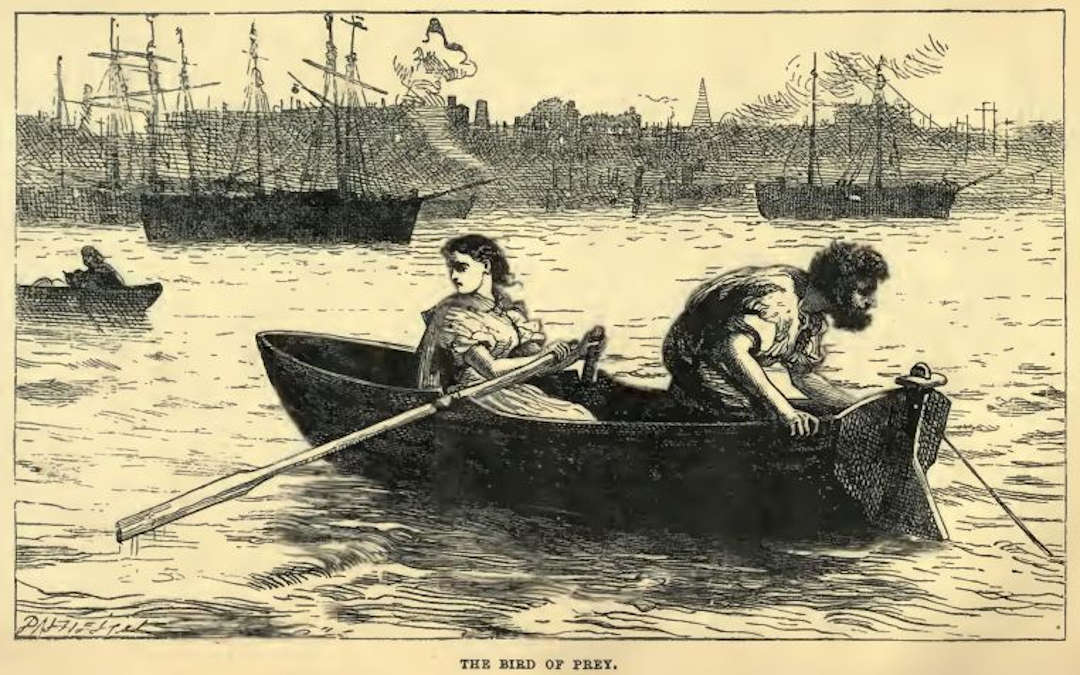
\includegraphics[scale=2.3]{01-01-01}

The school at which young Charley Hexam had first learned from a
book--the streets being, for pupils of his degree, the great Preparatory
Establishment in which very much that is never unlearned is learned
without and before book--was a miserable loft in an unsavoury yard. Its
atmosphere was oppressive and disagreeable; it was crowded, noisy,
and confusing; half the pupils dropped asleep, or fell into a state of
waking stupefaction; the other half kept them in either condition by
maintaining a monotonous droning noise, as if they were performing, out
of time and tune, on a ruder sort of bagpipe. The teachers, animated
solely by good intentions, had no idea of execution, and a lamentable
jumble was the upshot of their kind endeavours.

It was a school for all ages, and for both sexes. The latter were kept
apart, and the former were partitioned off into square assortments. But,
all the place was pervaded by a grimly ludicrous pretence that every
pupil was childish and innocent. This pretence, much favoured by the
lady-visitors, led to the ghastliest absurdities. Young women old in
the vices of the commonest and worst life, were expected to profess
themselves enthralled by the good child’s book, the Adventures of
Little Margery, who resided in the village cottage by the mill; severely
reproved and morally squashed the miller, when she was five and he was
fifty; divided her porridge with singing birds; denied herself a new
nankeen bonnet, on the ground that the turnips did not wear nankeen
bonnets, neither did the sheep who ate them; who plaited straw and
delivered the dreariest orations to all comers, at all sorts of
unseasonable times. So, unwieldy young dredgers and hulking mudlarks
were referred to the experiences of Thomas Twopence, who, having
resolved not to rob (under circumstances of uncommon atrocity) his
particular friend and benefactor, of eighteenpence, presently came into
supernatural possession of three and sixpence, and lived a shining light
ever afterwards. (Note, that the benefactor came to no good.) Several
swaggering sinners had written their own biographies in the same strain;
it always appearing from the lessons of those very boastful persons,
that you were to do good, not because it WAS good, but because you were
to make a good thing of it. Contrariwise, the adult pupils were taught
to read (if they could learn) out of the New Testament; and by dint of
stumbling over the syllables and keeping their bewildered eyes on the
particular syllables coming round to their turn, were as absolutely
ignorant of the sublime history, as if they had never seen or heard of
it. An exceedingly and confoundingly perplexing jumble of a school,
in fact, where black spirits and grey, red spirits and white, jumbled
jumbled jumbled jumbled, jumbled every night. And particularly every
Sunday night. For then, an inclined plane of unfortunate infants would
be handed over to the prosiest and worst of all the teachers with good
intentions, whom nobody older would endure. Who, taking his stand on
the floor before them as chief executioner, would be attended by a
conventional volunteer boy as executioner’s assistant. When and where it
first became the conventional system that a weary or inattentive infant
in a class must have its face smoothed downward with a hot hand, or when
and where the conventional volunteer boy first beheld such system in
operation, and became inflamed with a sacred zeal to administer it,
matters not. It was the function of the chief executioner to hold forth,
and it was the function of the acolyte to dart at sleeping infants,
yawning infants, restless infants, whimpering infants, and smooth their
wretched faces; sometimes with one hand, as if he were anointing them
for a whisker; sometimes with both hands, applied after the fashion of
blinkers. And so the jumble would be in action in this department for a
mortal hour; the exponent drawling on to My Dearert Childerrenerr, let
us say, for example, about the beautiful coming to the Sepulchre; and
repeating the word Sepulchre (commonly used among infants) five hundred
times, and never once hinting what it meant; the conventional boy
smoothing away right and left, as an infallible commentary; the whole
hot-bed of flushed and exhausted infants exchanging measles, rashes,
whooping-cough, fever, and stomach disorders, as if they were assembled
in High Market for the purpose.

Even in this temple of good intentions, an exceptionally sharp boy
exceptionally determined to learn, could learn something, and, having
learned it, could impart it much better than the teachers; as being
more knowing than they, and not at the disadvantage in which they stood
towards the shrewder pupils. In this way it had come about that Charley
Hexam had risen in the jumble, taught in the jumble, and been received
from the jumble into a better school.

‘So you want to go and see your sister, Hexam?’

‘If you please, Mr Headstone.’

‘I have half a mind to go with you. Where does your sister live?’

‘Why, she is not settled yet, Mr Headstone. I’d rather you didn’t see
her till she is settled, if it was all the same to you.’

‘Look here, Hexam.’ Mr Bradley Headstone, highly certificated
stipendiary schoolmaster, drew his right forefinger through one of the
buttonholes of the boy’s coat, and looked at it attentively. ‘I hope
your sister may be good company for you?’

‘Why do you doubt it, Mr Headstone?’

‘I did not say I doubted it.’

‘No, sir; you didn’t say so.’

Bradley Headstone looked at his finger again, took it out of the
buttonhole and looked at it closer, bit the side of it and looked at it
again.

‘You see, Hexam, you will be one of us. In good time you are sure to
pass a creditable examination and become one of us. Then the question
is--’

The boy waited so long for the question, while the schoolmaster looked
at a new side of his finger, and bit it, and looked at it again, that at
length the boy repeated:

‘The question is, sir--?’

‘Whether you had not better leave well alone.’

‘Is it well to leave my sister alone, Mr Headstone?’

‘I do not say so, because I do not know. I put it to you. I ask you to
think of it. I want you to consider. You know how well you are doing
here.’

‘After all, she got me here,’ said the boy, with a struggle.

‘Perceiving the necessity of it,’ acquiesced the schoolmaster, ‘and
making up her mind fully to the separation. Yes.’

The boy, with a return of that former reluctance or struggle or whatever
it was, seemed to debate with himself. At length he said, raising his
eyes to the master’s face:

‘I wish you’d come with me and see her, Mr Headstone, though she is not
settled. I wish you’d come with me, and take her in the rough, and judge
her for yourself.’

‘You are sure you would not like,’ asked the schoolmaster, ‘to prepare
her?’

‘My sister Lizzie,’ said the boy, proudly, ‘wants no preparing, Mr
Headstone. What she is, she is, and shows herself to be. There’s no
pretending about my sister.’

His confidence in her, sat more easily upon him than the indecision with
which he had twice contended. It was his better nature to be true to
her, if it were his worse nature to be wholly selfish. And as yet the
better nature had the stronger hold.

‘Well, I can spare the evening,’ said the schoolmaster. ‘I am ready to
walk with you.’

‘Thank you, Mr Headstone. And I am ready to go.’

Bradley Headstone, in his decent black coat and waistcoat, and decent
white shirt, and decent formal black tie, and decent pantaloons of
pepper and salt, with his decent silver watch in his pocket and its
decent hair-guard round his neck, looked a thoroughly decent young man
of six-and-twenty. He was never seen in any other dress, and yet there
was a certain stiffness in his manner of wearing this, as if there were
a want of adaptation between him and it, recalling some mechanics in
their holiday clothes. He had acquired mechanically a great store of
teacher’s knowledge. He could do mental arithmetic mechanically, sing
at sight mechanically, blow various wind instruments mechanically, even
play the great church organ mechanically. From his early childhood up,
his mind had been a place of mechanical stowage. The arrangement of
his wholesale warehouse, so that it might be always ready to meet the
demands of retail dealers history here, geography there, astronomy to
the right, political economy to the left--natural history, the physical
sciences, figures, music, the lower mathematics, and what not, all in
their several places--this care had imparted to his countenance a look
of care; while the habit of questioning and being questioned had given
him a suspicious manner, or a manner that would be better described as
one of lying in wait. There was a kind of settled trouble in the face.
It was the face belonging to a naturally slow or inattentive intellect
that had toiled hard to get what it had won, and that had to hold it now
that it was gotten. He always seemed to be uneasy lest anything should
be missing from his mental warehouse, and taking stock to assure
himself.

Suppression of so much to make room for so much, had given him a
constrained manner, over and above. Yet there was enough of what was
animal, and of what was fiery (though smouldering), still visible in
him, to suggest that if young Bradley Headstone, when a pauper lad, had
chanced to be told off for the sea, he would not have been the last man
in a ship’s crew. Regarding that origin of his, he was proud, moody, and
sullen, desiring it to be forgotten. And few people knew of it.

In some visits to the Jumble his attention had been attracted to this
boy Hexam. An undeniable boy for a pupil-teacher; an undeniable boy
to do credit to the master who should bring him on. Combined with this
consideration, there may have been some thought of the pauper lad now
never to be mentioned. Be that how it might, he had with pains gradually
worked the boy into his own school, and procured him some offices to
discharge there, which were repaid with food and lodging. Such were the
circumstances that had brought together, Bradley Headstone and young
Charley Hexam that autumn evening. Autumn, because full half a year had
come and gone since the bird of prey lay dead upon the river-shore.

The schools--for they were twofold, as the sexes--were down in that
district of the flat country tending to the Thames, where Kent and
Surrey meet, and where the railways still bestride the market-gardens
that will soon die under them. The schools were newly built, and there
were so many like them all over the country, that one might have thought
the whole were but one restless edifice with the locomotive gift of
Aladdin’s palace. They were in a neighbourhood which looked like a toy
neighbourhood taken in blocks out of a box by a child of particularly
incoherent mind, and set up anyhow; here, one side of a new street;
there, a large solitary public-house facing nowhere; here, another
unfinished street already in ruins; there, a church; here, an immense
new warehouse; there, a dilapidated old country villa; then, a medley
of black ditch, sparkling cucumber-frame, rank field, richly cultivated
kitchen-garden, brick viaduct, arch-spanned canal, and disorder of
frowziness and fog. As if the child had given the table a kick, and gone
to sleep.

But, even among school-buildings, school-teachers, and school-pupils,
all according to pattern and all engendered in the light of the latest
Gospel according to Monotony, the older pattern into which so many
fortunes have been shaped for good and evil, comes out. It came out in
Miss Peecher the schoolmistress, watering her flowers, as Mr Bradley
Headstone walked forth. It came out in Miss Peecher the schoolmistress,
watering the flowers in the little dusty bit of garden attached to her
small official residence, with little windows like the eyes in needles,
and little doors like the covers of school-books.

Small, shining, neat, methodical, and buxom was Miss Peecher;
cherry-cheeked and tuneful of voice. A little pincushion, a little
housewife, a little book, a little workbox, a little set of tables and
weights and measures, and a little woman, all in one. She could write
a little essay on any subject, exactly a slate long, beginning at the
left-hand top of one side and ending at the right-hand bottom of the
other, and the essay should be strictly according to rule. If Mr Bradley
Headstone had addressed a written proposal of marriage to her, she would
probably have replied in a complete little essay on the theme exactly a
slate long, but would certainly have replied Yes. For she loved him. The
decent hair-guard that went round his neck and took care of his decent
silver watch was an object of envy to her. So would Miss Peecher have
gone round his neck and taken care of him. Of him, insensible. Because
he did not love Miss Peecher.

Miss Peecher’s favourite pupil, who assisted her in her little
household, was in attendance with a can of water to replenish her little
watering-pot, and sufficiently divined the state of Miss Peecher’s
affections to feel it necessary that she herself should love young
Charley Hexam. So, there was a double palpitation among the double
stocks and double wall-flowers, when the master and the boy looked over
the little gate.

‘A fine evening, Miss Peecher,’ said the Master.

‘A very fine evening, Mr Headstone,’ said Miss Peecher. ‘Are you taking
a walk?’

‘Hexam and I are going to take a long walk.’

‘Charming weather,’ remarked Miss Peecher, ‘FOR a long walk.’

‘Ours is rather on business than mere pleasure,’ said the Master. Miss
Peecher inverting her watering-pot, and very carefully shaking out the
few last drops over a flower, as if there were some special virtue in
them which would make it a Jack’s beanstalk before morning, called for
replenishment to her pupil, who had been speaking to the boy.

‘Good-night, Miss Peecher,’ said the Master.

‘Good-night, Mr Headstone,’ said the Mistress.

The pupil had been, in her state of pupilage, so imbued with the
class-custom of stretching out an arm, as if to hail a cab or omnibus,
whenever she found she had an observation on hand to offer to Miss
Peecher, that she often did it in their domestic relations; and she did
it now.

‘Well, Mary Anne?’ said Miss Peecher.

‘If you please, ma’am, Hexam said they were going to see his sister.’

‘But that can’t be, I think,’ returned Miss Peecher: ‘because Mr
Headstone can have no business with HER.’

Mary Anne again hailed.

‘Well, Mary Anne?’

‘If you please, ma’am, perhaps it’s Hexam’s business?’

‘That may be,’ said Miss Peecher. ‘I didn’t think of that. Not that it
matters at all.’

Mary Anne again hailed.

‘Well, Mary Anne?’

‘They say she’s very handsome.’

‘Oh, Mary Anne, Mary Anne!’ returned Miss Peecher, slightly colouring
and shaking her head, a little out of humour; ‘how often have I told you
not to use that vague expression, not to speak in that general way? When
you say THEY say, what do you mean? Part of speech They?’

Mary Anne hooked her right arm behind her in her left hand, as being
under examination, and replied:

‘Personal pronoun.’

‘Person, They?’

‘Third person.’

‘Number, They?’

‘Plural number.’

‘Then how many do you mean, Mary Anne? Two? Or more?’

‘I beg your pardon, ma’am,’ said Mary Anne, disconcerted now she came
to think of it; ‘but I don’t know that I mean more than her brother
himself.’ As she said it, she unhooked her arm.

‘I felt convinced of it,’ returned Miss Peecher, smiling again. ‘Now
pray, Mary Anne, be careful another time. He says is very different from
they say, remember. Difference between he says and they say? Give it
me.’

Mary Anne immediately hooked her right arm behind her in her left
hand--an attitude absolutely necessary to the situation--and replied:
‘One is indicative mood, present tense, third person singular, verb
active to say. Other is indicative mood, present tense, third person
plural, verb active to say.’

‘Why verb active, Mary Anne?’

‘Because it takes a pronoun after it in the objective case, Miss
Peecher.’

‘Very good indeed,’ remarked Miss Peecher, with encouragement. ‘In fact,
could not be better. Don’t forget to apply it, another time, Mary Anne.’
This said, Miss Peecher finished the watering of her flowers, and
went into her little official residence, and took a refresher of the
principal rivers and mountains of the world, their breadths, depths, and
heights, before settling the measurements of the body of a dress for her
own personal occupation.

Bradley Headstone and Charley Hexam duly got to the Surrey side of
Westminster Bridge, and crossed the bridge, and made along the Middlesex
shore towards Millbank. In this region are a certain little street
called Church Street, and a certain little blind square, called Smith
Square, in the centre of which last retreat is a very hideous church
with four towers at the four corners, generally resembling some
petrified monster, frightful and gigantic, on its back with its legs
in the air. They found a tree near by in a corner, and a blacksmith’s
forge, and a timber yard, and a dealer’s in old iron. What a rusty
portion of a boiler and a great iron wheel or so meant by lying
half-buried in the dealer’s fore-court, nobody seemed to know or to want
to know. Like the Miller of questionable jollity in the song, They cared
for Nobody, no not they, and Nobody cared for them.

After making the round of this place, and noting that there was a deadly
kind of repose on it, more as though it had taken laudanum than fallen
into a natural rest, they stopped at the point where the street and the
square joined, and where there were some little quiet houses in a row.
To these Charley Hexam finally led the way, and at one of these stopped.

‘This must be where my sister lives, sir. This is where she came for a
temporary lodging, soon after father’s death.’

‘How often have you seen her since?’

‘Why, only twice, sir,’ returned the boy, with his former reluctance;
‘but that’s as much her doing as mine.’

‘How does she support herself?’

‘She was always a fair needlewoman, and she keeps the stockroom of a
seaman’s outfitter.’

‘Does she ever work at her own lodging here?’

‘Sometimes; but her regular hours and regular occupation are at their
place of business, I believe, sir. This is the number.’

The boy knocked at a door, and the door promptly opened with a spring
and a click. A parlour door within a small entry stood open, and
disclosed a child--a dwarf--a girl--a something--sitting on a little low
old-fashioned arm-chair, which had a kind of little working bench before
it.

‘I can’t get up,’ said the child, ‘because my back’s bad, and my legs
are queer. But I’m the person of the house.’

‘Who else is at home?’ asked Charley Hexam, staring.

‘Nobody’s at home at present,’ returned the child, with a glib assertion
of her dignity, ‘except the person of the house. What did you want,
young man?’

‘I wanted to see my sister.’

‘Many young men have sisters,’ returned the child. ‘Give me your name,
young man?’

The queer little figure, and the queer but not ugly little face, with
its bright grey eyes, were so sharp, that the sharpness of the manner
seemed unavoidable. As if, being turned out of that mould, it must be
sharp.

‘Hexam is my name.’

‘Ah, indeed?’ said the person of the house. ‘I thought it might be. Your
sister will be in, in about a quarter of an hour. I am very fond of your
sister. She’s my particular friend. Take a seat. And this gentleman’s
name?’

‘Mr Headstone, my schoolmaster.’

‘Take a seat. And would you please to shut the street door first? I
can’t very well do it myself; because my back’s so bad, and my legs are
so queer.’

They complied in silence, and the little figure went on with its work of
gumming or gluing together with a camel’s-hair brush certain pieces
of cardboard and thin wood, previously cut into various shapes. The
scissors and knives upon the bench showed that the child herself had cut
them; and the bright scraps of velvet and silk and ribbon also strewn
upon the bench showed that when duly stuffed (and stuffing too was
there), she was to cover them smartly. The dexterity of her nimble
fingers was remarkable, and, as she brought two thin edges accurately
together by giving them a little bite, she would glance at the visitors
out of the corners of her grey eyes with a look that out-sharpened all
her other sharpness.

‘You can’t tell me the name of my trade, I’ll be bound,’ she said, after
taking several of these observations.

‘You make pincushions,’ said Charley.

‘What else do I make?’

‘Pen-wipers,’ said Bradley Headstone.

‘Ha! ha! What else do I make? You’re a schoolmaster, but you can’t tell
me.’

‘You do something,’ he returned, pointing to a corner of the little
bench, ‘with straw; but I don’t know what.’

‘Well done you!’ cried the person of the house. ‘I only make pincushions
and pen-wipers, to use up my waste. But my straw really does belong to
my business. Try again. What do I make with my straw?’

‘Dinner-mats?’

‘A schoolmaster, and says dinner-mats! I’ll give you a clue to my trade,
in a game of forfeits. I love my love with a B because she’s Beautiful;
I hate my love with a B because she is Brazen; I took her to the sign of
the Blue Boar, and I treated her with Bonnets; her name’s Bouncer, and
she lives in Bedlam.--Now, what do I make with my straw?’

‘Ladies’ bonnets?’

‘Fine ladies’,’ said the person of the house, nodding assent. ‘Dolls’.
I’m a Doll’s Dressmaker.’

‘I hope it’s a good business?’

The person of the house shrugged her shoulders and shook her head. ‘No.
Poorly paid. And I’m often so pressed for time! I had a doll married,
last week, and was obliged to work all night. And it’s not good for me,
on account of my back being so bad and my legs so queer.’

They looked at the little creature with a wonder that did not diminish,
and the schoolmaster said: ‘I am sorry your fine ladies are so
inconsiderate.’

‘It’s the way with them,’ said the person of the house, shrugging her
shoulders again. ‘And they take no care of their clothes, and they
never keep to the same fashions a month. I work for a doll with three
daughters. Bless you, she’s enough to ruin her husband!’ The person of
the house gave a weird little laugh here, and gave them another look out
of the corners of her eyes. She had an elfin chin that was capable of
great expression; and whenever she gave this look, she hitched this chin
up. As if her eyes and her chin worked together on the same wires.

‘Are you always as busy as you are now?’

‘Busier. I’m slack just now. I finished a large mourning order the day
before yesterday. Doll I work for, lost a canary-bird.’ The person of
the house gave another little laugh, and then nodded her head several
times, as who should moralize, ‘Oh this world, this world!’

‘Are you alone all day?’ asked Bradley Headstone. ‘Don’t any of the
neighbouring children--?’

‘Ah, lud!’ cried the person of the house, with a little scream, as
if the word had pricked her. ‘Don’t talk of children. I can’t bear
children. I know their tricks and their manners.’ She said this with an
angry little shake of her tight fist close before her eyes.

Perhaps it scarcely required the teacher-habit, to perceive that the
doll’s dressmaker was inclined to be bitter on the difference between
herself and other children. But both master and pupil understood it so.

‘Always running about and screeching, always playing and fighting,
always skip-skip-skipping on the pavement and chalking it for their
games! Oh! I know their tricks and their manners!’ Shaking the little
fist as before. ‘And that’s not all. Ever so often calling names in
through a person’s keyhole, and imitating a person’s back and legs. Oh!
I know their tricks and their manners. And I’ll tell you what I’d do, to
punish ‘em. There’s doors under the church in the Square--black doors,
leading into black vaults. Well! I’d open one of those doors, and I’d
cram ‘em all in, and then I’d lock the door and through the keyhole I’d
blow in pepper.’

‘What would be the good of blowing in pepper?’ asked Charley Hexam.

‘To set ‘em sneezing,’ said the person of the house, ‘and make their
eyes water. And when they were all sneezing and inflamed, I’d mock ‘em
through the keyhole. Just as they, with their tricks and their manners,
mock a person through a person’s keyhole!’

An uncommonly emphatic shake of her little fist close before her eyes,
seemed to ease the mind of the person of the house; for she added
with recovered composure, ‘No, no, no. No children for me. Give me
grown-ups.’

It was difficult to guess the age of this strange creature, for her poor
figure furnished no clue to it, and her face was at once so young and so
old. Twelve, or at the most thirteen, might be near the mark.

‘I always did like grown-ups,’ she went on, ‘and always kept company
with them. So sensible. Sit so quiet. Don’t go prancing and capering
about! And I mean always to keep among none but grown-ups till I marry.
I suppose I must make up my mind to marry, one of these days.’

She listened to a step outside that caught her ear, and there was a soft
knock at the door. Pulling at a handle within her reach, she said,
with a pleased laugh: ‘Now here, for instance, is a grown-up that’s my
particular friend!’ and Lizzie Hexam in a black dress entered the room.

‘Charley! You!’

Taking him to her arms in the old way--of which he seemed a little
ashamed--she saw no one else.

‘There, there, there, Liz, all right my dear. See! Here’s Mr Headstone
come with me.’

Her eyes met those of the schoolmaster, who had evidently expected
to see a very different sort of person, and a murmured word or two
of salutation passed between them. She was a little flurried by the
unexpected visit, and the schoolmaster was not at his ease. But he never
was, quite.

‘I told Mr Headstone you were not settled, Liz, but he was so kind as to
take an interest in coming, and so I brought him. How well you look!’

Bradley seemed to think so.

‘Ah! Don’t she, don’t she?’ cried the person of the house, resuming her
occupation, though the twilight was falling fast. ‘I believe you she
does! But go on with your chat, one and all:

\begin{verbatim}
     You one two three,
     My com-pa-nie,
     And don’t mind me.’
\end{verbatim}

--pointing this impromptu rhyme with three points of her thin
fore-finger.

‘I didn’t expect a visit from you, Charley,’ said his sister. ‘I
supposed that if you wanted to see me you would have sent to me,
appointing me to come somewhere near the school, as I did last time.
I saw my brother near the school, sir,’ to Bradley Headstone, ‘because
it’s easier for me to go there, than for him to come here. I work about
midway between the two places.’

‘You don’t see much of one another,’ said Bradley, not improving in
respect of ease.

‘No.’ With a rather sad shake of her head. ‘Charley always does well, Mr
Headstone?’

‘He could not do better. I regard his course as quite plain before him.’

‘I hoped so. I am so thankful. So well done of you, Charley dear! It is
better for me not to come (except when he wants me) between him and his
prospects. You think so, Mr Headstone?’

Conscious that his pupil-teacher was looking for his answer, that he
himself had suggested the boy’s keeping aloof from this sister, now seen
for the first time face to face, Bradley Headstone stammered:

‘Your brother is very much occupied, you know. He has to work hard. One
cannot but say that the less his attention is diverted from his work,
the better for his future. When he shall have established himself, why
then--it will be another thing then.’

Lizzie shook her head again, and returned, with a quiet smile: ‘I always
advised him as you advise him. Did I not, Charley?’

‘Well, never mind that now,’ said the boy. ‘How are you getting on?’

‘Very well, Charley. I want for nothing.’

‘You have your own room here?’

‘Oh yes. Upstairs. And it’s quiet, and pleasant, and airy.’

‘And she always has the use of this room for visitors,’ said the
person of the house, screwing up one of her little bony fists, like an
opera-glass, and looking through it, with her eyes and her chin in that
quaint accordance. ‘Always this room for visitors; haven’t you, Lizzie
dear?’

It happened that Bradley Headstone noticed a very slight action of
Lizzie Hexam’s hand, as though it checked the doll’s dressmaker. And it
happened that the latter noticed him in the same instant; for she made
a double eyeglass of her two hands, looked at him through it, and cried,
with a waggish shake of her head: ‘Aha! Caught you spying, did I?’

It might have fallen out so, any way; but Bradley Headstone also noticed
that immediately after this, Lizzie, who had not taken off her bonnet,
rather hurriedly proposed that as the room was getting dark they should
go out into the air. They went out; the visitors saying good-night to
the doll’s dressmaker, whom they left, leaning back in her chair with
her arms crossed, singing to herself in a sweet thoughtful little voice.

‘I’ll saunter on by the river,’ said Bradley. ‘You will be glad to talk
together.’

As his uneasy figure went on before them among the evening shadows, the
boy said to his sister, petulantly:

‘When are you going to settle yourself in some Christian sort of place,
Liz? I thought you were going to do it before now.’

‘I am very well where I am, Charley.’

‘Very well where you are! I am ashamed to have brought Mr Headstone with
me. How came you to get into such company as that little witch’s?’

‘By chance at first, as it seemed, Charley. But I think it must have
been by something more than chance, for that child--You remember the
bills upon the walls at home?’

‘Confound the bills upon the walls at home! I want to forget the bills
upon the walls at home, and it would be better for you to do the same,’
grumbled the boy. ‘Well; what of them?’

‘This child is the grandchild of the old man.’

‘What old man?’

‘The terrible drunken old man, in the list slippers and the night-cap.’

The boy asked, rubbing his nose in a manner that half expressed vexation
at hearing so much, and half curiosity to hear more: ‘How came you to
make that out? What a girl you are!’

‘The child’s father is employed by the house that employs me; that’s how
I came to know it, Charley. The father is like his own father, a weak
wretched trembling creature, falling to pieces, never sober. But a good
workman too, at the work he does. The mother is dead. This poor ailing
little creature has come to be what she is, surrounded by drunken people
from her cradle--if she ever had one, Charley.’

‘I don’t see what you have to do with her, for all that,’ said the boy.

‘Don’t you, Charley?’

The boy looked doggedly at the river. They were at Millbank, and
the river rolled on their left. His sister gently touched him on the
shoulder, and pointed to it.

‘Any compensation--restitution--never mind the word, you know my
meaning. Father’s grave.’

But he did not respond with any tenderness. After a moody silence he
broke out in an ill-used tone:

‘It’ll be a very hard thing, Liz, if, when I am trying my best to get up
in the world, you pull me back.’

‘I, Charley?’

‘Yes, you, Liz. Why can’t you let bygones be bygones? Why can’t you, as
Mr Headstone said to me this very evening about another matter, leave
well alone? What we have got to do, is, to turn our faces full in our
new direction, and keep straight on.’

‘And never look back? Not even to try to make some amends?’

‘You are such a dreamer,’ said the boy, with his former petulance. ‘It
was all very well when we sat before the fire--when we looked into the
hollow down by the flare--but we are looking into the real world, now.’

‘Ah, we were looking into the real world then, Charley!’

‘I understand what you mean by that, but you are not justified in it. I
don’t want, as I raise myself to shake you off, Liz. I want to carry you
up with me. That’s what I want to do, and mean to do. I know what I owe
you. I said to Mr Headstone this very evening, “After all, my sister got
me here.” Well, then. Don’t pull me back, and hold me down. That’s all I
ask, and surely that’s not unconscionable.’

She had kept a steadfast look upon him, and she answered with composure:

‘I am not here selfishly, Charley. To please myself I could not be too
far from that river.’

‘Nor could you be too far from it to please me. Let us get quit of it
equally. Why should you linger about it any more than I? I give it a
wide berth.’

‘I can’t get away from it, I think,’ said Lizzie, passing her hand
across her forehead. ‘It’s no purpose of mine that I live by it still.’

‘There you go, Liz! Dreaming again! You lodge yourself of your own
accord in a house with a drunken--tailor, I suppose--or something of the
sort, and a little crooked antic of a child, or old person, or whatever
it is, and then you talk as if you were drawn or driven there. Now, do
be more practical.’

She had been practical enough with him, in suffering and striving
for him; but she only laid her hand upon his shoulder--not
reproachfully--and tapped it twice or thrice. She had been used to
do so, to soothe him when she carried him about, a child as heavy as
herself. Tears started to his eyes.

‘Upon my word, Liz,’ drawing the back of his hand across them, ‘I mean
to be a good brother to you, and to prove that I know what I owe you.
All I say is, that I hope you’ll control your fancies a little, on my
account. I’ll get a school, and then you must come and live with me,
and you’ll have to control your fancies then, so why not now? Now, say I
haven’t vexed you.’

‘You haven’t, Charley, you haven’t.’

‘And say I haven’t hurt you.’

‘You haven’t, Charley.’ But this answer was less ready.

‘Say you are sure I didn’t mean to. Come! There’s Mr Headstone stopping
and looking over the wall at the tide, to hint that it’s time to go.
Kiss me, and tell me that you know I didn’t mean to hurt you.’

She told him so, and they embraced, and walked on and came up with the
schoolmaster.

‘But we go your sister’s way,’ he remarked, when the boy told him he was
ready. And with his cumbrous and uneasy action he stiffly offered her
his arm. Her hand was just within it, when she drew it back. He looked
round with a start, as if he thought she had detected something that
repelled her, in the momentary touch.

‘I will not go in just yet,’ said Lizzie. ‘And you have a distance
before you, and will walk faster without me.’

Being by this time close to Vauxhall Bridge, they resolved, in
consequence, to take that way over the Thames, and they left her;
Bradley Headstone giving her his hand at parting, and she thanking him
for his care of her brother.

The master and the pupil walked on, rapidly and silently. They had
nearly crossed the bridge, when a gentleman came coolly sauntering
towards them, with a cigar in his mouth, his coat thrown back, and his
hands behind him. Something in the careless manner of this person,
and in a certain lazily arrogant air with which he approached, holding
possession of twice as much pavement as another would have claimed,
instantly caught the boy’s attention. As the gentleman passed the boy
looked at him narrowly, and then stood still, looking after him.

‘Who is it that you stare after?’ asked Bradley.

‘Why!’ said the boy, with a confused and pondering frown upon his face,
‘It IS that Wrayburn one!’

Bradley Headstone scrutinized the boy as closely as the boy had
scrutinized the gentleman.

‘I beg your pardon, Mr Headstone, but I couldn’t help wondering what in
the world brought HIM here!’

Though he said it as if his wonder were past--at the same time resuming
the walk--it was not lost upon the master that he looked over his
shoulder after speaking, and that the same perplexed and pondering frown
was heavy on his face.

‘You don’t appear to like your friend, Hexam?’

‘I DON’T like him,’ said the boy.

‘Why not?’

‘He took hold of me by the chin in a precious impertinent way, the first
time I ever saw him,’ said the boy.

‘Again, why?’

‘For nothing. Or--it’s much the same--because something I happened to
say about my sister didn’t happen to please him.’

‘Then he knows your sister?’

‘He didn’t at that time,’ said the boy, still moodily pondering.

‘Does now?’

The boy had so lost himself that he looked at Mr Bradley Headstone
as they walked on side by side, without attempting to reply until the
question had been repeated; then he nodded and answered, ‘Yes, sir.’

‘Going to see her, I dare say.’

‘It can’t be!’ said the boy, quickly. ‘He doesn’t know her well enough.
I should like to catch him at it!’

When they had walked on for a time, more rapidly than before, the master
said, clasping the pupil’s arm between the elbow and the shoulder with
his hand:

‘You were going to tell me something about that person. What did you say
his name was?’

‘Wrayburn. Mr Eugene Wrayburn. He is what they call a barrister, with
nothing to do. The first time he came to our old place was when my
father was alive. He came on business; not that it was HIS business--HE
never had any business--he was brought by a friend of his.’

‘And the other times?’

‘There was only one other time that I know of. When my father was killed
by accident, he chanced to be one of the finders. He was mooning about,
I suppose, taking liberties with people’s chins; but there he was,
somehow. He brought the news home to my sister early in the morning, and
brought Miss Abbey Potterson, a neighbour, to help break it to her.
He was mooning about the house when I was fetched home in the
afternoon--they didn’t know where to find me till my sister could be
brought round sufficiently to tell them--and then he mooned away.’

‘And is that all?’

‘That’s all, sir.’

Bradley Headstone gradually released the boy’s arm, as if he were
thoughtful, and they walked on side by side as before. After a long
silence between them, Bradley resumed the talk.

‘I suppose--your sister--’ with a curious break both before and after
the words, ‘has received hardly any teaching, Hexam?’

‘Hardly any, sir.’

‘Sacrificed, no doubt, to her father’s objections. I remember them in
your case. Yet--your sister--scarcely looks or speaks like an ignorant
person.’

‘Lizzie has as much thought as the best, Mr Headstone. Too much,
perhaps, without teaching. I used to call the fire at home, her books,
for she was always full of fancies--sometimes quite wise fancies,
considering--when she sat looking at it.’

‘I don’t like that,’ said Bradley Headstone.

His pupil was a little surprised by this striking in with so sudden
and decided and emotional an objection, but took it as a proof of the
master’s interest in himself. It emboldened him to say:

‘I have never brought myself to mention it openly to you, Mr Headstone,
and you’re my witness that I couldn’t even make up my mind to take it
from you before we came out to-night; but it’s a painful thing to think
that if I get on as well as you hope, I shall be--I won’t say disgraced,
because I don’t mean disgraced--but--rather put to the blush if it was
known--by a sister who has been very good to me.’

‘Yes,’ said Bradley Headstone in a slurring way, for his mind scarcely
seemed to touch that point, so smoothly did it glide to another, ‘and
there is this possibility to consider. Some man who had worked his way
might come to admire--your sister--and might even in time bring himself
to think of marrying--your sister--and it would be a sad drawback and a
heavy penalty upon him, if; overcoming in his mind other inequalities of
condition and other considerations against it, this inequality and this
consideration remained in full force.’

‘That’s much my own meaning, sir.’

‘Ay, ay,’ said Bradley Headstone, ‘but you spoke of a mere brother.
Now, the case I have supposed would be a much stronger case; because an
admirer, a husband, would form the connexion voluntarily, besides being
obliged to proclaim it: which a brother is not. After all, you know, it
must be said of you that you couldn’t help yourself: while it would be
said of him, with equal reason, that he could.’

‘That’s true, sir. Sometimes since Lizzie was left free by father’s
death, I have thought that such a young woman might soon acquire more
than enough to pass muster. And sometimes I have even thought that
perhaps Miss Peecher--’

‘For the purpose, I would advise Not Miss Peecher,’ Bradley Headstone
struck in with a recurrence of his late decision of manner.

‘Would you be so kind as to think of it for me, Mr Headstone?’

‘Yes, Hexam, yes. I’ll think of it. I’ll think maturely of it. I’ll
think well of it.’

Their walk was almost a silent one afterwards, until it ended at the
school-house. There, one of neat Miss Peecher’s little windows, like the
eyes in needles, was illuminated, and in a corner near it sat Mary Anne
watching, while Miss Peecher at the table stitched at the neat little
body she was making up by brown paper pattern for her own wearing. N.B.
Miss Peecher and Miss Peecher’s pupils were not much encouraged in the
unscholastic art of needlework, by Government.

Mary Anne with her face to the window, held her arm up.

‘Well, Mary Anne?’

‘Mr Headstone coming home, ma’am.’

In about a minute, Mary Anne again hailed.

‘Yes, Mary Anne?’

‘Gone in and locked his door, ma’am.’

Miss Peecher repressed a sigh as she gathered her work together for bed,
and transfixed that part of her dress where her heart would have been if
she had had the dress on, with a sharp, sharp needle.



